
% Include LaTeX packages
\documentclass[conference]{styles/acmsiggraph}
\usepackage{fullpage}
\usepackage{enumitem}
\usepackage{amsmath,amsthm,amssymb}
\usepackage{listings}
\usepackage{graphicx}
\usepackage{etoolbox}
\usepackage{verbatim}
\usepackage[dvipsnames]{xcolor}
\usepackage{fancyvrb}
\usepackage{hyperref}
\usepackage{menukeys}
\usepackage{booktabs}
% \setlength{\parskip}{0.4em}

\title{Assignment 1: Solutions \\ {IS711: Learning and Planning in Intelligent Systems}}
\author{SHI Jieke \\ jkshi.2022@phdcs.smu.edu.sg}
\pdfauthor{SHI Jieke}

\begin{document}
\maketitle
\vspace{-0.15cm}
\section{Question \#1}

\subsection{Answer to Question \#1.1}

We can formulate the problem with the following definitions:
The state space is the set of all possible configurations.
\begin{itemize}[itemsep=0.1em, leftmargin=*]
	\setlength{\itemsep}{0pt}
	\setlength{\parsep}{0pt}
	\setlength{\parskip}{0pt}
	\item \textbf{State representation}: A state can be represented by two piles. Each pile is represented by a stack of blocks denoted as color+label. For example, the Configuration 1 of this question is in the state of \{[\textit{Green A, Grey B, Orange A}], [\textit{Yellow B, Green C}]\}. There are five blocks available. The first block of each pile is the top and the last block is on the table.
	\item \textbf{State space}: The state space is the set of all possible configurations of two piles.
	\item \textbf{Initial state}: \{[\textit{Green A, Grey B, Orange A}], [\textit{Yellow B, Green C}]\}.
	\item \textbf{Goal state}: \{[\textit{Green C, Grey B, Yellow B, Orange A, Green A}], []\}.
	\item \textbf{Possible Operators}: denoting $x$ and $y$ as two blocks, the possible operators are:
	\begin{itemize}
		\item \textit{Move(x, y)}: move a block from the top of a pile to the top of another pile.
		\item \textit{MoveToTable(x)}: move a block from the top of a pile to the table.
	\end{itemize}
	\item \textbf{Path cost}: The cost of each call to operator \textit{Move(x, y)} is 1. The cost of each call to operator \textit{MoveToTable(x)} is determined by color, namely, Orange block costs 2, Gray block costs 3, Yellow block costs 1, Green block costs 4. The path cost is the sum of the costs of all operators.
\end{itemize}

\subsection{Answer to Question \#1.2}
In the initial state con0, we can do the operation moveTo(2,1), moveToTable(2), moveTo(1,2), 
moveToTable(1), and get different configurations respectively, con1, con2, con3, con4, based 
on the formula f(n) = g(n) + h(n), we can get the estimated the cost of each configuration and 

The first four nodes in the search tree are shown in Figure~\ref{}.

We could design a n as the amount of blocks that are not above the right block. 

This heuristic value n is the number of blocks that are not above the right block. Because it always smaller or equal to the real cost, since when even one block still not in right place, it will take at least one operation to adjust its position. 

Therefore, h(u) is equal or smaller than real cost. It is admissible.



\section{Question \#2}

The trip with the least possible cost would need 6 large buses and 5 small buses.
The calculation using linear programming is as follows:
\begin{itemize}[leftmargin=*]
	\setlength{\itemsep}{0pt}
	\setlength{\parsep}{0pt}
	\setlength{\parskip}{0pt}
	\item \textbf{Variables}: $x_1$: the number of large buses; $x_2$: the number of small buses.
	\item \textbf{Objective}: Minimize rental costs, i.e.,
	\begin{equation}
		\min 800x_1 + 600 x_2
	\end{equation}
	\item \textbf{Constraints}: Subject to the following constraints:
	\begin{equation}
		\begin{aligned}
			& 50x_1 + 40x_2 \geq 500 \\
			& x_1 + x_2 \leq 11 \\
			& 0 \leq x_1 \leq 10 \\
			& 0 \leq x_2 \leq 8 \\
		\end{aligned}
	\end{equation}
	\item \textbf{Solution}: As shown in Figure~\ref{fig:2}, the optimal solution is $x_1 = 6$ and $x_2 = 5$. The minimum cost is $800 \times 6 + 600 \times 5 = 7800$.
	\begin{figure}
		\centering
		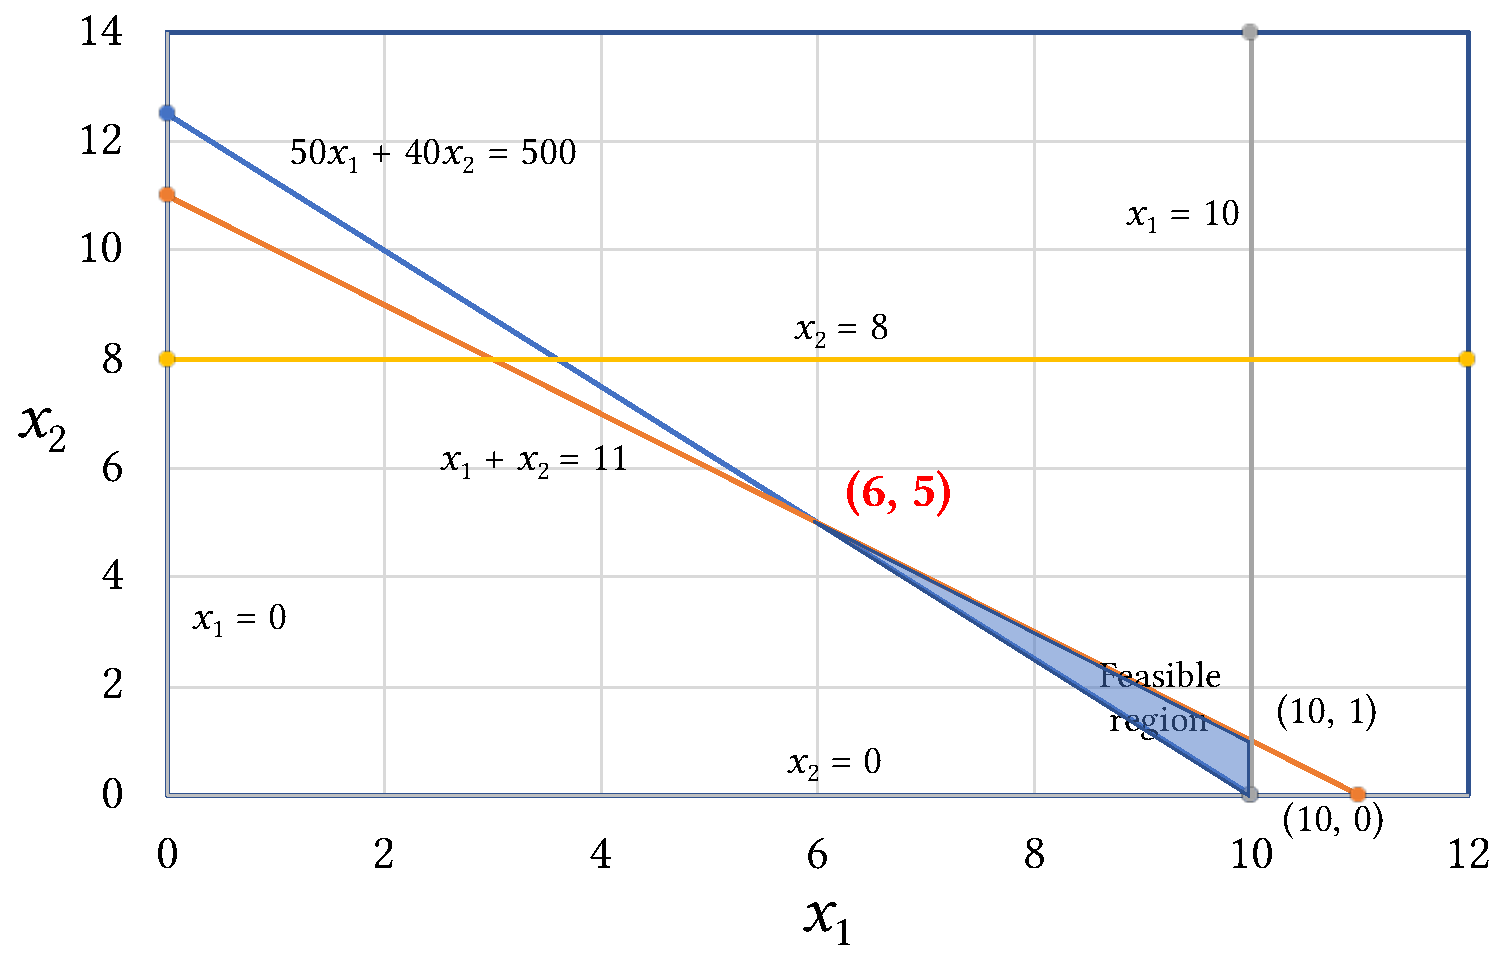
\includegraphics[width=0.7\textwidth]{figures/q2.pdf}
		\caption{Solution to Question \#2}
		\label{fig:2}
	\end{figure}
\end{itemize}

The drawbacks of linear programming are:
\begin{itemize}
	\setlength{\itemsep}{0pt}
	\setlength{\parsep}{0pt}
	\setlength{\parskip}{0pt}
    \item To the above question, we can observe redundant computation in linear programming, i.e., if we remove the constraint $x_2\leq 8$, the answer will be unchanged. The other constraints are already sufficient conditions for the answer, but linear programming still needs to compute the redundant constraint $x_2\leq 8$.
    \item In the general cases of using linear programming, 
    \begin{itemize}
        \item  When facing real-life problems, it is possible that the constraints may not be directly expressible as linear inequalities. Non-linear relations may be involved, e.g., $x_1^2 + x_2^2 \leq 100$;
        \item When solving linear programming, there is no guarantee of getting integer values. A non-integer valued solution will be meaningless to lots of problems.
        \item Linear programming can only handle single-objective problems, while real-life decision-making problems often have multiple objectives.
        \item The solution of linear programming can involve massive mathematical calculations. In some cases, the solution may not be available due to the complexity of the problem.
	\end{itemize}
\end{itemize}

\section{Question \#3}

I will play the game as the winning probability is $0.517 > 0.5$, and the expected value is $0.279 > 0$. The calculation is as follows:

For each round of rolling the dice, there exist $6^3$ possible outcomes. Among them, 
\begin{itemize}
	\setlength{\itemsep}{0pt}
	\setlength{\parsep}{0pt}
	\setlength{\parskip}{0pt}
	\item There is 1 outcome whose total is 3. 
	\item There are 10 outcomes whose total is 6.
	\item There are 21 outcomes whose total is 8.
	\item There are 25 outcomes whose total is 9.
	\item There are 27 outcomes whose total is 11.
	\item There are 25 outcomes whose total is 12.
	\item There are 10 outcomes whose total is 15.
	\item There are 1 outcomes whose total is 18.
\end{itemize}

Therefore, the probability of winning \$1 in the first round is
\begin{equation}
	P(\text{winning \$1 in first round}) = \frac{1+21+27+10}{6^3} = \frac{59}{216} \approx 0.273
\end{equation}

The probability of losing \$1 in the first round is
\begin{equation}
	P(\text{losing \$1 in first round}) = \frac{25+1}{6^3} = \frac{26}{216} \approx 0.120
\end{equation}

% The probability of playing one more time is
% \begin{equation} 
% 	P(\text{playing one more time}) = 1- \frac{59}{216} - \frac{26}{216}  = \frac{131}{216} \approx 0.606
% \end{equation}

The probability of winning \$2 in the second round is
\begin{equation} 
	P(\text{winning \$2 in second round}) = (1- \frac{59}{216} - \frac{26}{216}) \times \frac{10+25+27+25}{6^3} = \frac{11397}{46656} \approx 0.244
\end{equation}

The probability of losing \$1 in the second round is
\begin{equation} 
	P(\text{losing \$1 in the second round}) = 1- \frac{59}{216} - \frac{26}{216}- \frac{11397}{46656} = \frac{16899}{46656}  \approx 0.362
\end{equation}

Thus, the winning probability of this game is
\begin{equation}
	P(\text{winning}) = 0.273+0.244 = 0.517 > 0.5
\end{equation}
The expected value of the game is
\begin{equation}
	E = \frac{59}{216} \times 1 + \frac{26}{216} \times (-1) + \frac{11397}{46656} \times 2 + \frac{16899}{46656} \times (-1) =  \frac{13023}{46656} \approx 0.279 > 0 
\end{equation}

The winning probability is $0.517 > 0.5$, and the expected value is $0.279 > 0$, thus, I will play the game.

\section{Question \#4}

\subsection{Answer to Question \#4.1}

\subsection{Answer to Question \#4.2}

\subsection{Answer to Question \#4.3}

\section{Question \#5}

\section{Question \#6}

\subsection{Answer to Question \#6.a}

There are 4 states, S = (L1, L2, L3, L4).
Actions, A = (“wait to pick up a custom”, “MoveToL1”, “MoveToL1”, “MoveToL2”, “MoveToL3”, “MoveToL4”)
Reward function's value are shows as below table


\subsection{Answer to Question \#6.b}

\end{document}
